\section{Условие задания}

Согласно порядковому номеру в списке 13 принимаем схему I и номер варианта 7.

\begin{figure}[H]
    \begin{center}
        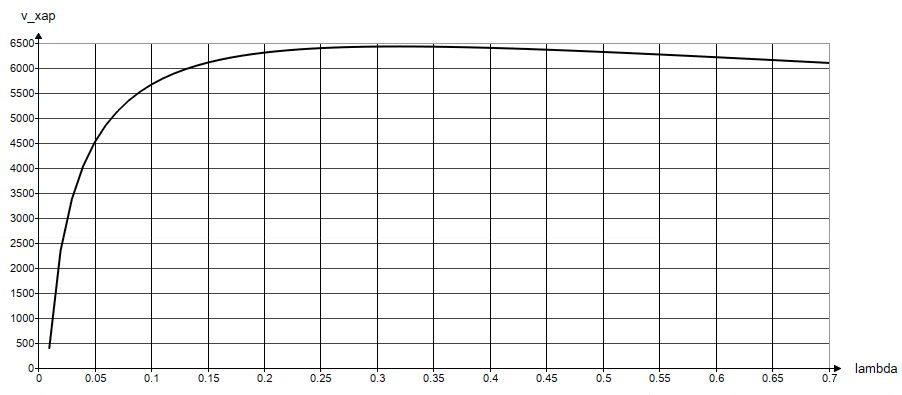
\includegraphics[width = 0.9\linewidth]{pic1.PNG}
        \caption{Схема ракеты}
        \label{pic1}
    \end{center}
\end{figure}

Исходные данные:
\begin{itemize}
    \item Координаты сечения 
        \begin{itemize}
        \item $x_1 = 1.7$ м
        \item $x_2 = 3.5$ м
        \item $x_3 = 4.0$ м
        \item $x_4 = 7.0$ м
        \item $x_5 = 10.0$ м
        \item $x_6 = 11.0$ м
        \item $x_7 = 15.0$ м
        \item $x_8 = 19.0$ м
        \item $x_9 = 21.0$ м
    \end{itemize}
    \item Параметры АС
        \begin{itemize}
            \item $\omega_0 = 25 \t{с}^{-1}$
            \item $\omega_\pi = 70 \t{с}^{-1}$
            \item $\omega_{2\pi} = 110 \t{с}^{-1}$
            \item $k_\t{р} = 0.6$
        \end{itemize}
    \item $M_1 = 2.0$ т
    \item $M_2 = 2.0$ т
    \item $J_0 = 3.0 \; \t{т} \cdot \t{м}^2$
    \item $x_\t{ГП} = 19.5$ м
\end{itemize}

При выполнении ДЗ №2 использовать результаты ДЗ №1.

В задании требуется:
\begin{enumerate}
    \item Используя <<универсальную диаграмму устойчивости>> оценить устойчивость движения упругой ракеты по траектории.
    \item Если полученный ответ отрицательный (движение неустойчиво), то:
    \begin{itemize}
        \item уточнить границы смежной области неустойчивости
        \item предъявить требования в АС.
    \end{itemize}
    \item Если полученный ответ положительный (движение устойчиво), то необходимо уточнить границы неустойчивости смежных областей.
\end{enumerate}

При расчетах полагать, что $\epsilon = 0.001$.

Градиент управляющей силы вычислить по формуле: $R_\t{ур} = k_p \cdot M_0 \cdot g_0$ \\
где $M_0$ --- стартовая масса, $g_0$ --- ускорение свободного падения, $k_p$ --- коэффициент, заданный в таблице.

Амплитуду АС для частоты большей, чем частота среза вычислять по формуле: $A_\t{АС} = 0.5 \cdot \exp(0.01 \cdot (\omega_0 - \omega))$

\vspace{10pt}

$\displaystyle \phi_\t{АС} = -\pi \frac{\omega_0 - \omega}{\omega_0 - \omega_\pi}$ для $\omega_0 < \omega < \omega_\pi$;

\vspace{10pt}

$\displaystyle \phi_\t{АС} = -\pi - \pi \frac{\omega_\pi - \omega}{\omega_\pi - \omega_{2\pi}}$ для $\omega_\pi < \omega < \omega_{2\pi}$

\section{Оценка устойчивости движения упругой ракеты по траектории с помощью <<универсальной диаграммы устойчивости>>}

\begin{figure}[H]
    \begin{center}
        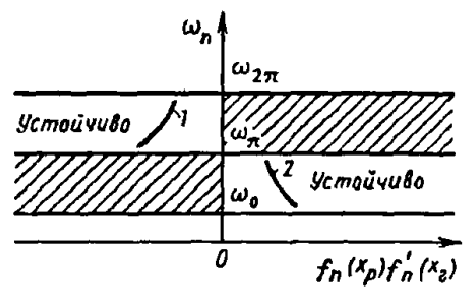
\includegraphics[width = 0.5\linewidth]{pic2.PNG}
        \caption{Универсальная диаграмма устойчивости}
        \label{pic2}
    \end{center}
\end{figure}

Для того, чтобы параметры объекта регулирования были расположены в области устойчивости, необходимо, чтобы выполнялись следующие условия:
\begin{enumerate}
    \item Для первого тона колебаний $f_n(x_\t{р}) \cdot f_n'(x_\t{ГП}) > 0$
    \item Для второго тона колебаний $f_n(x_\t{р}) \cdot f_n'(x_\t{ГП}) < 0$
    \item $\omega_0 < \omega_1 < \omega_\pi$
    \item $\omega_\pi < \omega_2 < \omega_{2\pi}$
\end{enumerate}

Проверим условия:
\begin{enumerate}
    \item $f_1(x_\t{р}) \cdot f_1'(x_\t{ГП}) = 0.045 > 0$ --- условие выполнено
    \item $f_2(x_\t{р}) \cdot f_2'(x_\t{ГП}) = 2.331 > 0$ --- условие не выполнено
    \item $25 < 12.11 < 70$ --- условие не выполнено
    \item $70 < 34.974 < 110$ --- условие не выполнено
\end{enumerate}

Значит ракета не устойчива.

\section{Уточнение границы смежной области неустойчивости}

Найдем собственные частоты первых двух тонов колебаний ракеты по мере ее опустошения. Зададим шаг заполнения баков топливом $5\%$.

\begin{table}[H]
    \caption{Результаты расчетов для различных степеней заполнения баков}
    \label{tab1}
    \begin{center}
        \begin{tabular}{|c|c|c|c|c|}
            \hline
            Доля заполнения баков $s$ & $\omega_1$ & $f_1(x_\t{р}) \cdot f_1'(x_\t{ГП})$ & $\omega_2$ & $f_2(x_\t{р}) \cdot f_2'(x_\t{ГП})$ \\
            \hline
            1 & 10.289 & 0.096 & 25.009 & 0.186 \\
            \hline
            0.95 & 10.593 & 0.087 & 25.097 & 0.193 \\ 
            \hline
            0.9 & 10.878 & 0.079 & 25.254 & 0.214 \\ 
            \hline
            0.85 & 11.138 & 0.072 & 25.532 & 0.252 \\ 
            \hline
            0.8 & 11.366 & 0.065 & 25.984 & 0.315 \\ 
            \hline
            0.75 & 11.557 & 0.059 & 26.657 & 0.412 \\ 
            \hline
            0.7 & 11.713 & 0.054 & 27.597 & 0.562 \\ 
            \hline
            0.65 & 11.836 & 0.05 & 28.85 & 0.788 \\ 
            \hline
            0.6 & 11.935 & 0.047 & 30.461 & 1.126 \\ 
            \hline
            0.55 & 12.022 & 0.045 & 32.482 & 1.622 \\ 
            \hline
            0.5 & 12.11 & 0.045 & 34.974 & 2.331 \\ 
            \hline
            0.45 & 12.214 & 0.046 & 38.002 & 3.308 \\ 
            \hline
            0.4 & 12.355 & 0.048 & 41.636 & 4.583 \\ 
            \hline
            0.35 & 12.553 & 0.052 & 45.932 & 6.114 \\ 
            \hline
            0.3 & 12.842 & 0.058 & 50.902 & 7.725 \\ 
            \hline
            0.25 & 13.268 & 0.067 & 56.47 & 9.064 \\ 
            \hline
            0.2 & 13.913 & 0.083 & 62.413 & 9.642 \\ 
            \hline
            0.15 & 14.934 & 0.107 & 68.333 & 9.046 \\ 
            \hline
            0.1 & 16.703 & 0.153 & 73.762 & 7.202 \\ 
            \hline
            0.05 & 20.423 & 0.249 & 78.785 & 4.318 \\ 
            \hline
            0 & 34.831 & 0.632 & 94.88 & 0.487 \\
            \hline
        \end{tabular}
    \end{center}
\end{table}

\begin{figure}[H]
    \begin{center}
        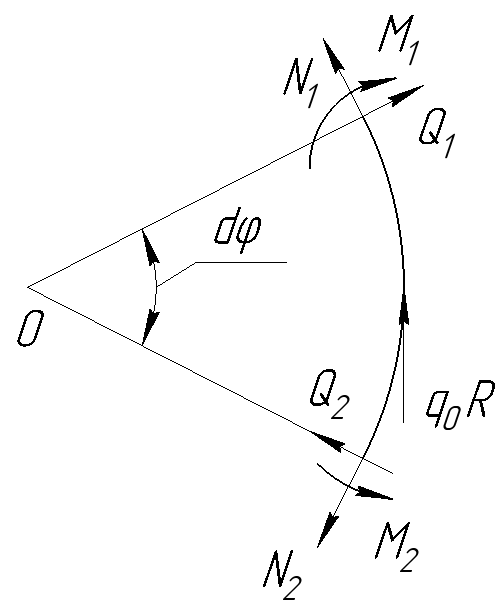
\includegraphics[width = 0.7\linewidth]{pic3.PNG}
        \caption{Диаграмма устойчивости для первого тона}
        \label{pic3}
    \end{center}
\end{figure}
\begin{figure}[H]
    \begin{center}
        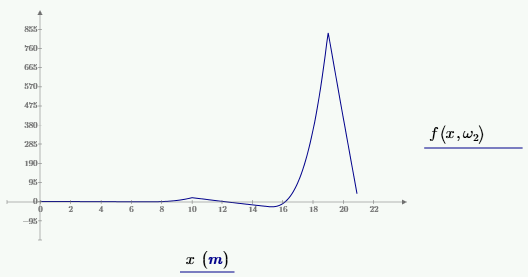
\includegraphics[width = 0.7\linewidth]{pic4.PNG}
        \caption{Диаграмма устойчивости для второго тона}
        \label{pic4}
    \end{center}
\end{figure}

Условие $\omega_0 < \omega_1 < \omega_\pi$ для первого тона колебаний выполяется только при $s < 0.05$. На остальном участке ракета является неустойчивой по первому тону. Для второго тона колебаний условие $\omega_\pi < \omega_2 < \omega_{2\pi}$ выполняется только на участке $s < 0.15$. Это значит, что ракета устойчива только при заполненности топливом $s < 0.05$. Найдем более точную границу.

При $s = 0.02298$ $\displaystyle \omega_1 = 25 \; \frac{\t{рад}}{\t{с}}$; $\displaystyle \omega_2 = 82.741 \; \frac{\t{рад}}{\t{с}}$. Этой заполненности соответствуют координаты зеркал комнонентов топлива: $x_4 = 9.862 \; \t{м}$, $x_7 = 18.816 \; \t{м}$.

При этом для второго тона колебаний выражение $f_n(x_\t{р}) \cdot f_n'(x_\t{ГП}) > 0$, что соответствует неустойчивой ракете. Поэтому необходимо сместить положение гироплатформы.

\section{Предъявление требований к АС}

Для определения положения гироплатформы введем вспомогательную функцию $\phi(x) = f_n(x) \cdot f_n'(x)$. Построим ее график для второго тона колебаний для граничного значения $s = 0.02298$, значения $s = 0.2$, соответствующего максимальному значению $\phi_n(x)$ и для полностью заправленной ракеты:
\begin{figure}[H]
    \begin{center}
        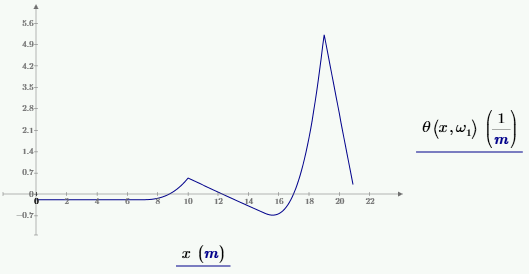
\includegraphics[width = \linewidth]{pic5.PNG}
        \caption{График $\phi_n(x)$ при разном уровне заполненности}
        \label{pic5}
    \end{center}
\end{figure}

Как видно из графика, функция $\phi_n(x)$ принимает отрицательное значение при $9 \; \t{м} < x < 13 \; \t{м}$. Поскольку межбаковый отсек располагается по координатам от $x_5 = 10 \; \t{м}$ до $x_6 = 11 \; \t{м}$ целесообразно разместить гироплатформу в нем. Построим диаграмму устойчивости для расположения гироплатформы в точке $x = 10.5 \; \t{м}$.
\begin{figure}[H]
    \begin{center}
        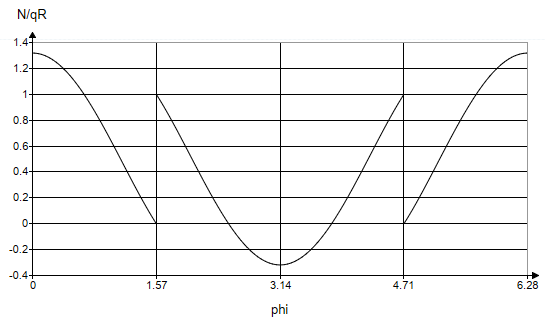
\includegraphics[width = 0.7\linewidth]{pic6.PNG}
        \caption{Диаграмма устойчивости}
        \label{pic6}
    \end{center}
\end{figure}
\begin{figure}[H]
    \begin{center}
        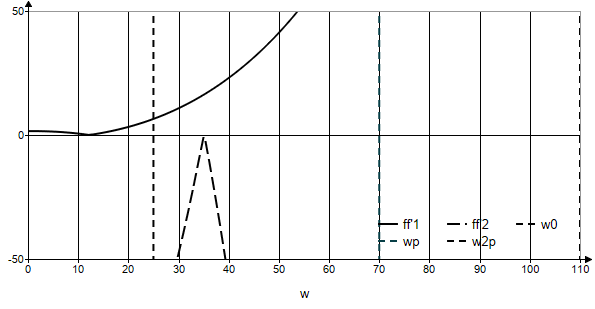
\includegraphics[width = 0.7\linewidth]{pic7.PNG}
        \caption{Диаграмма устойчивости в области оси $\omega$}
        \label{pic7}
    \end{center}
\end{figure}